\chapter{Background and Related Work}
\label{ch:background}

    \section{Computing Continuum}
    \label{sec:computing-continuum-background}

        Placeholder

    \section{Scheduling and Adaptation}
    \label{sec:scheduling-and-adaptation-background}

    \section{Prediction of Load}
    \label{sec:prediction-of-load-background}

    \section{Recurrent Neural Network}
    \label{sec:rnn-background}


        Recurrent neural networks (RNN) were designed to improve upon the shortcomings of traditional neural networks when dealing with sequential data.
        
        
        \subsection{Recurrent Cell Architecture}
        \label{sec:recurrent-cell-architecture-background}

            A traditional feed-forward neural network (FNN) is unidirectional, meaning that they have a single direction and hence cannot persist information over a time step $t$.
            Looping structures are added to a feed-forward neural network that enable the persistance of information about time-series or sequential data. 
            This is the reason RNN's are known as "recurrent" neural networks.
            \begin{figure}[h!]
                \centering
                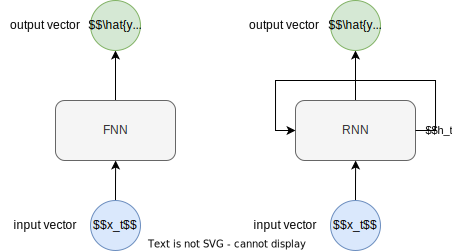
\includegraphics[scale=0.5]{figures/FNN_vs_RNN.drawio.png}
                \caption{FNN vs. RNN}
                \label{fig:fnn-vs-rnn}
            \end{figure}
            As can be seen in figure \ref{fig:fnn-vs-rnn}, the RNN has an additional loop inside it to persist time-series information. The loop structure enables the RNN to apply a \emph{recurrence relation} (see \ref{sec:recurrence-relation-background}) at every time step in order to process a sequence.

            The rectangle containing the "RNN" label is defined as a "recurrent cell".
            This workflow of a single RNN cell can be seen in more detail in figure \ref{fig:single-rnn-cell}, where the previous cell state $h_{t-1}$ and the current input $x_t$ are used as the input of the recurrent cell, get combined and forwarded to the $tanh$ \emph{activation function}, which returns the output vector $\hat{y}_t$ and $h_t$ (the recurrence relation).

        \subsection{Recurrence Relation}
        \label{sec:recurrence-relation-background}

            The recurrence relation is applied at every time step to process a sequence.

            The recurrent relation seen in figures \ref{fig:fnn-vs-rnn}, \ref{fig:single-rnn-cell} is denoted as $h_t$, and is defined as $h_t = f_w(h_{t - 1}, x_t)$, where $f_w$ is a function that is parametrized by the weights, $h_{t-1}$ is the previous state and $x_t$ is the input vector at time step $t$. With the addition of $h_{t-1}$, the model is now also taking the previous time step into account when updating the current time step. 
            \begin{figure}[h!]
                \centering
                \includegraphics[scale=0.5]{figures/single_rnn_cell.drawio.png}
                \caption{Single RNN Cell}
                \label{fig:single-rnn-cell}
            \end{figure}

            The recurrence relation in a more mathematical notation is:

            $$h_t = \tanh(W^T_{hh} h_{t-1} + W^T_{xh} x_t)$$
            
            Both the input vector $x_t$ as well as the previous state $h_{t-1}$ are multiplied with the two separate weight matrices $W^T_{xh}$ and $W^T{hh}$ respectively, combined and fed to the $\tanh$ activation function. Finally, the $\tanh$ function returns the output vector $\hat{y}_t$ at time step $t$.

        \subsection{RNN Loop Unfolding}
        \label{sec:rnn-loop-unfolding-background}

            The loop unfolding will provide a description about how RNN handle sequential data at every time step.
            As can  e seen in figure \ref{fig:rnn-loop-unfolding}, the model is adding the input at every time step, and generating an output $\hat{y}_i$ for every time step.
            The weight matrices $W_{hh}$ that are used for every time step for updating the previous state are the same for every time step.
            The weight matrix $W_{xh}$ is applied to every $x_i$ and is also the same for every time step $i$.

            \begin{figure}[h!]
                \centering
                \includegraphics[width=0.90\textwidth]{figures/rnn_loop_unfolding.drawio.png}
                \caption{RNN Loop Unfolding}
                \label{fig:rnn-loop-unfolding}
            \end{figure}
            \begin{itemize}[label=\textemdash]
                \item $x_i$ denotes the input value at time step $i$.
                \item $\hat{y}_i$ denotes the output value at time step $i$.
                \item $W_{hh}$ denotes the weight matrix to update the previous state.
                \item $W_{xh}$ denotes the weight matrix that is applied to the input value at every time step.
            \end{itemize}
            The output vectors $\hat{y}_0, \hat{y}_1, \hat{y}_2, \dots, \hat{y}_t$ can be used to calculate the separate losses $L_0, L_1, L_2, \dots, L_t$ at each time step $t$.
            % This completes the forward propagation (see \ref{sec:forward-propagation}).

        \subsection{Loss Calculation and Weight Updates for RNN}
        \label{sec:loss-calculation-and-weight-updates-for-rnn-background}

            The loss is defined as $L = L_0, L_1, \dots, L_t$

        \subsection{Common Problems of RNNs}
        \label{sec:shortcomings-of-rnns-background}

            Regularly experienced problems of RNNs are the exploding or vanishing gradient problems.
            \begin{quote}
                The motivation behind why they happen is that it is hard to catch long haul conditions as a result of a multiplicative angle that can be dramatically diminishing/expanding regarding the number of layers. \cite{parikhDisadvantagesRNN2021}
            \end{quote}
            These problems occur when the sequence is too long and this may result in the model training with either null weights (i.e. the model won't learn while training) or exploding weights.
            
            
            \paragraph{Exploding Gradients}
            \label{par:exploding-gradients-background}

                The Exploding Gradients problem occurs when many of the values (i.e. weight matrices, or gradients themselves) involved in the repeated gradient computations are greater than 1. 
                If this is the case, then gradients become extremely large and optimising them becomes computationally intensive.
                To solve the Exploding Gradients problem, a process called \emph{Gradient Clipping} is applied, that scales the gradient values to smaller values less than 1.


            \paragraph{Vanishing Gradients}
            \label{par:vanishing-gradients-background}

                The Vanishing Gradients problem occurs when many of the values (i.e. weight matrices or gradients themselves) that are involved in the repeated gradient computations are too small or less than 1. Opposed to the \nameref{par:exploding-gradients-background} problem, the gradients become smaller with each repeated computation of the gradients.
                This results in the problem of \emph{long term dependency}, were smaller sequences can be remembered and the weights updated accordingly. But for longer sequences, the model will unlikely be able to yield a good prediction performance.

                There are multiple solutions to the Vanishing Gradient problem, such as changing the activation function from $\tanh$ to \emph{Rectified Linear Unit (ReLU)}. Also initialising the weights of the model can solve this problem, though tailored heuristics (such as the \emph{Xavier Weight Initialisation}) should be used to result in omitting the Vanishing Gradients problem and also increase the efficiency of the training. Another solution is to change the architecture of the neural network and adding more complex recurrent units that are mentioned in section \ref{sec:lstm-background}.

    \section{Long-Short Term Memory}
    \label{sec:lstm-background}

        \emph{Long-Short Term Memory (LSTM)} are a type of \ref{sec:rnn-background} but improve upon the shortcomings of regular RNN models.
        LSTMs are best suited for learning long term dependencies in sequential or time-series data.

        The introduction of \emph{self-looping} to produce paths is the main architectural improvement for LSTMs over RNNs. This additional component diminishes the problem of the vanishing gradients problem and enables gradients to flow for a long duration.

    % \section{Forward-Propagation}
    % \label{sec:forward-propagation}
        
    %     Placeholder

    % \section{Backward-Propagation}

    % \section{Activation Function}

    % \section{Loss Function}


    \section{Public Cloud Provider Traces in Available Data}
    \label{sec:public-cloud-provider-traces-in-available-data-sota}

    \section{Resource Prediction based on Machine Learning}
    \label{sec:resource-prediction-based-on-machine-learning-sota}